%%%%%%%%%%%%%%%%%%%%%%%%%%%%%%%%%%%%%%%%%%%%%%%%%%%%%%%%%%%%%%%%%%%%%%%%%%%%%%%%%%%%%%%%%%%%%%%%%%%%%%%%%%%%%%%%%%%%%%%%%%%%%%%%%%%%%%%%%%%%%%%%%%%%%%%%%%%%%%%%%%%
% Written By Michael Brodskiy
% Class: Quantum Mechanics
% Professor: G. Fiete
%%%%%%%%%%%%%%%%%%%%%%%%%%%%%%%%%%%%%%%%%%%%%%%%%%%%%%%%%%%%%%%%%%%%%%%%%%%%%%%%%%%%%%%%%%%%%%%%%%%%%%%%%%%%%%%%%%%%%%%%%%%%%%%%%%%%%%%%%%%%%%%%%%%%%%%%%%%%%%%%%%%

\documentclass[12pt]{article} 
\usepackage{alphalph}
\usepackage[utf8]{inputenc}
\usepackage[russian,english]{babel}
\usepackage{titling}
\usepackage{amsmath}
\usepackage{float}
\usepackage{graphicx}
\usepackage{enumitem}
\usepackage{amssymb}
\usepackage[super]{nth}
\usepackage{everysel}
\usepackage{ragged2e}
\usepackage{geometry}
\usepackage{multicol}
\usepackage{fancyhdr}
\usepackage{cancel}
\usepackage{siunitx}
\usepackage{physics}
\usepackage{tikz}
\usepackage{mathdots}
\usepackage{yhmath}
\usepackage{cancel}
\usepackage{color}
\usepackage{array}
\usepackage{multirow}
\usepackage{gensymb}
\usepackage{tabularx}
\usepackage{extarrows}
\usepackage{booktabs}
\usepackage{lastpage}
\usetikzlibrary{fadings}
\usetikzlibrary{patterns}
\usetikzlibrary{shadows.blur}
\usetikzlibrary{shapes}

\geometry{top=1.0in,bottom=1.0in,left=1.0in,right=1.0in}
\newcommand{\subtitle}[1]{%
  \posttitle{%
    \par\end{center}
    \begin{center}\large#1\end{center}
    \vskip0.5em}%

}
\usepackage{hyperref}
\hypersetup{
colorlinks=true,
linkcolor=blue,
filecolor=magenta,      
urlcolor=blue,
citecolor=blue,
}


\title{Homework 7}
\date{\today}
\author{Michael Brodskiy\\ \small Professor: G. Fiete}

\begin{document}

\maketitle

\begin{enumerate}

  \item We begin by writing out the eigenstates as:

    $$\ket{n}=\frac{1}{\sqrt{2\pi}}e^{in\phi}$$

    We may take the inner product of two \underline{different} states ($n\neq m$) to get:

    $$\bra{m}\ket{n}=\frac{1}{2\pi}\int_0^{2\pi}e^{i(n-m)\phi}\,d\phi$$

    We evaluate to get:

    $$\bra{m}\ket{n}=\frac{1}{2\pi i(n-m)}\left[e^{i(n-m)\phi}\right]\Big|_0^{2\pi}$$
    $$\bra{m}\ket{n}=\frac{1}{2\pi i(n-m)}\left[e^{2\pi i(n-m)}-1\right]$$

    Since the exponent is an integer multiple of $2\pi$, we get:

    $$\bra{m}\ket{n}=\frac{1}{2\pi i(n-m)}\left[1-1\right]$$
    $$\boxed{\bra{m}\ket{n}=0}$$

    Furthermore, the inner product of the same eigenstate gives us:

    $$\braket{n}=\frac{1}{2\pi}\int_0^{2\pi}\,d\phi$$
    $$\braket{n}=\frac{2\pi}{2\pi}$$
    $$\boxed{\braket{n}=1}$$

    Accordingly, we observe that \underline{the states are orthonormal}:

    $$\boxed{\bra{m}\ket{n}=\delta_{mn}}$$

  \item

    \begin{enumerate}

      \item We begin by normalizing:

        $$\braket{\psi}=\int_{0}^{2\pi}\Big|\frac{N}{2+\cos(3\phi)}\Big|^2\,d\phi$$

        We expand to get:

        $$\braket{\psi}=\int_{0}^{2\pi}\frac{|N|^2}{4+4\cos(3\phi)+\cos^2(3\phi)}\,d\phi$$

        Using a solver, we obtain:

        $$\braket{\psi}=|N^2|\left( \frac{4\pi}{3\sqrt{3}} \right)$$

        As such, we get:

        $$\boxed{N=\sqrt{\left(\frac{4\pi}{3\sqrt{3}}\right)^{-1}}}$$

        The wave function becomes:

        $$\boxed{\psi(\phi)=\left( \frac{4\pi}{3\sqrt{3}} \right)^{-1/2}\frac{1}{2+\cos(3\phi)}}$$

      \item We plot the function to get:

        \begin{figure}[H]
          \centering
          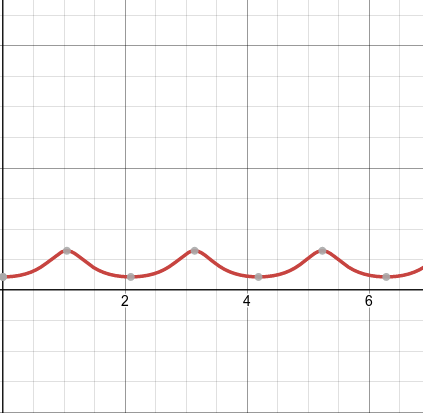
\includegraphics[width=.5\textwidth]{Figures/HW7-2b}
          \caption{Plot of $\psi(\phi)$}
          \label{fig:1}
        \end{figure}

      \item We may write the expectation value as:

        $$\langle L_z\rangle = \bra{\psi|L_z}\ket{\psi}$$

        This gives us:

        $$\bra{\psi|L_z}\ket{\psi}=\int_{0}^{2\pi} \psi^*(\phi) L_z\psi(\phi)\,d\phi$$

        We expand to get:

        $$\bra{\psi|L_z}\ket{\psi}=\left[\frac{4\pi}{3\sqrt{3}}\right]^{-1}\int_{0}^{2\pi}\frac{1}{2+\cos(3\phi)}\left( -i\hbar\frac{d}{d\phi} \right)\frac{1}{2+\cos(3\phi)} \,d\phi$$

        Now, we solve:

        $$\bra{\psi|L_z}\ket{\psi}=i\hbar\frac{ 3\sqrt{3}}{4\pi}\int_{0}^{2\pi}\frac{1}{2+\cos(3\phi)}\left[\frac{3\sin(3\phi)}{(2+\cos(3\phi))^2}\right] \,d\phi$$
        $$\bra{\psi|L_z}\ket{\psi}=i\hbar\frac{ 3\sqrt{3}}{4\pi}\int_{0}^{2\pi}\frac{3\sin(3\phi)}{(2+\cos(3\phi))^3} \,d\phi$$

        Entering this into a solver, we obtain:

        $$\boxed{\langle L_z\rangle=0}$$

        Evidently, we can see that the integrand must evaluate to zero, since, otherwise, the expectation value would be imaginary.

    \end{enumerate}

  \item For $l=1$, the spherical harmonics are:

    $$Y^0_1(\theta,\phi)=\sqrt{\frac{3}{4\pi}}\cos(\theta)$$
    $$Y^{-1}_1(\theta,\phi)=\sqrt{\frac{3}{8\pi}}\sin(\theta)e^{-i\phi}$$
    $$Y^{1}_1(\theta,\phi)=-\sqrt{\frac{3}{8\pi}}\sin(\theta)e^{i\phi}$$

    We expand to get:

    $$Y^{-1}_1(\theta,\phi)=\sqrt{\frac{3}{8\pi}}\sin(\theta)[\cos(\phi)-i\sin(\phi)]$$
    $$Y^{1}_1(\theta,\phi)=-\sqrt{\frac{3}{8\pi}}\sin(\theta)[\cos(\phi)+i\sin(\phi)]$$

    Finally, we transform from spherical to rectangular coordinates to get:

    $$\boxed{Y^0_1(x,y,z)=\sqrt{\frac{3}{4\pi}}\frac{z}{\sqrt{x^2+y^2+z^2}}}$$
    $$\boxed{Y^{-1}_1(x,y,z)=\sqrt{\frac{3}{8\pi}}\frac{x-iy}{\sqrt{x^2+y^2+z^2}}}$$
    $$\boxed{Y^{1}_1(x,y,z)=-\sqrt{\frac{3}{8\pi}}\frac{x+iy}{\sqrt{x^2+y^2+z^2}}}$$

    Combining the $m=\pm1$ functions, gives us $x$ or $y$ in the numerator:

    $$\boxed{\frac{1}{\sqrt{2}}\left[ Y^{-1}_1-Y^{1}_1 \right]=\sqrt{\frac{3}{4\pi}}\frac{x}{\sqrt{x^2+y^2+z^2}}}$$
    $$\boxed{\frac{1}{\sqrt{2}}\left[ Y^{-1}_1+Y^{1}_1 \right]=\sqrt{\frac{3}{4\pi}}\frac{y}{\sqrt{x^2+y^2+z^2}}}$$

    We see that these form the real spherical harmonics, or the $p_x,p_y$, and $p_z$ orbitals.

\end{enumerate}

\end{document}

